\chapter{Background}
\label{cha:background}

This chapter aims to provide a general overview of the tools used while building CogniDriver. It also describes some basic concepts about how the brain works which would be useful to know before diving into the description of the headset. 

\section{Development tools}

\subsection{Unity}
Unity is a game engine which allows the user to import objects easily and have them automatically updated if the source file changes. One may also create primitive shapes such as spheres and cubes in order to build simple objects to which textures can be applied. All objects support affine transformations and Unity provides a good physics engine. It also allows scene design and collision detection between different components. The final product can be deployed on a variety of platforms.

We should also highlight some of the reasons why Unity was chosen in favour of other game engines such as UnReal. Unity allows file import by a simple drag-and-drop and it also auto-updates the objects if the source files are changed using another program (e.g. Paint, Photoshop). The advantages of UnReal over Unity would be better graphics (mainly lighting) and the fact that it can fracture meshes. In terms of scripting, Unity allows development in JavaScript, C\# and Boo, while UDK only allows UnrealScript. For CogniDriver, C\# has been the scripting language choice, because it allows Object Oriented Programming (OOP), it is scalable for larger projects and bugs are easier to track down. 

Unity has been used to create games such as Assassin's Creed Identity \cite{assassins} and Battlestar Galactica Online \cite{battlestar}.

\subsection{Easy Roads 3D}
This plugin is available in the Unity asset store. The free version has been used for this project. It allows placing markers through which the road should go, and given a specified width, it approximates corners and builds the rest of the road into a single layer.

\subsection{Photoshop}
A trial version has been used to create some materials and textures such as: skid marks, rain, smoke texture, speedometer, arrows, colour choice. None of these are difficult to create, but I like Photoshop because it is easy to use by both novice and professional users. In addition, the layers allow the user to create many compositions and modify the image at will.

\section{Electroencephalography (EEG)}
The neuron is the core component of the nervous system. More neurons can connect together to form synapses and when one of these cells is excited, an electrical signal is generated. The electrical signals can be amplified and the resulting waveforms, known as brainwaves, can thus be obtained. They can then be used to monitor the brain activity of a person in order to detect abnormalities. In table \ref{table:brainwaves}, a representation of each type of most common brainwaves is shown, together with the normal activities in which these occur most often. Data comes from \cite{wikiEEG}. %, but the values have been checked with those in other sources. Typically, a small difference in frequency might be present in different sources. 

\begin{table}[h]

\newcolumntype{C}{>{\centering\arraybackslash} m{2cm} }  %# New column type
                             
\begin{tabular}{ | C | C | C | m{8cm}C | }
\hline
\textbf{Name}  & \textbf{Frequency (Hz)} & \textbf{Occurs in} & \textbf{Image Representation} \\ \hline
Delta & \textless 4    & deep sleep , unconsciousness, deep anaesthesia, hypoxia          & 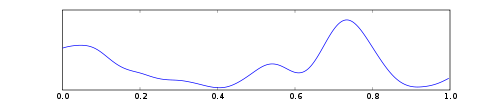
\includegraphics[scale=0.5]{500px-Eeg_delta.png}        \\ \hline
Theta & 4 - 7          & stress, unconsciousness, deep relaxation          & 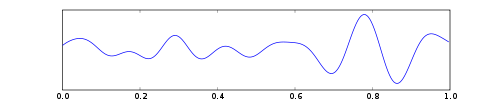
\includegraphics[scale=0.5]{500px-Eeg_theta.png}        \\ \hline
Alpha & 8 - 15         & relaxation          & 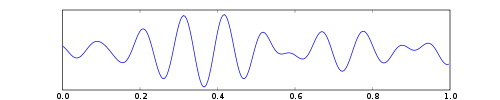
\includegraphics[scale=0.5]{500px-Eeg_alpha.png}        \\ \hline
Beta  & 16 - 31        & conciousness, alertness, thinking, sensory stimulation          & 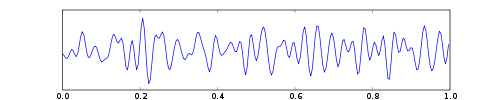
\includegraphics[scale=0.5]{500px-Eeg_beta.png}         \\ \hline
Gamma & 32 +           & selective attention, human cognition and perceptive activities         & 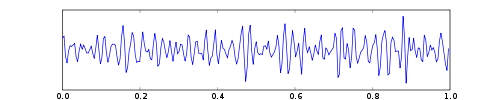
\includegraphics[scale=0.5]{500px-Eeg_gamma.png}        \\ \hline
\end{tabular}
\captionof{table} {Information about brainwaves types \cite{musicEEG}. Image Credit: Hugo Gamboa}
\label{table:brainwaves}

\end{table}

\begin{figure}
  \centering
  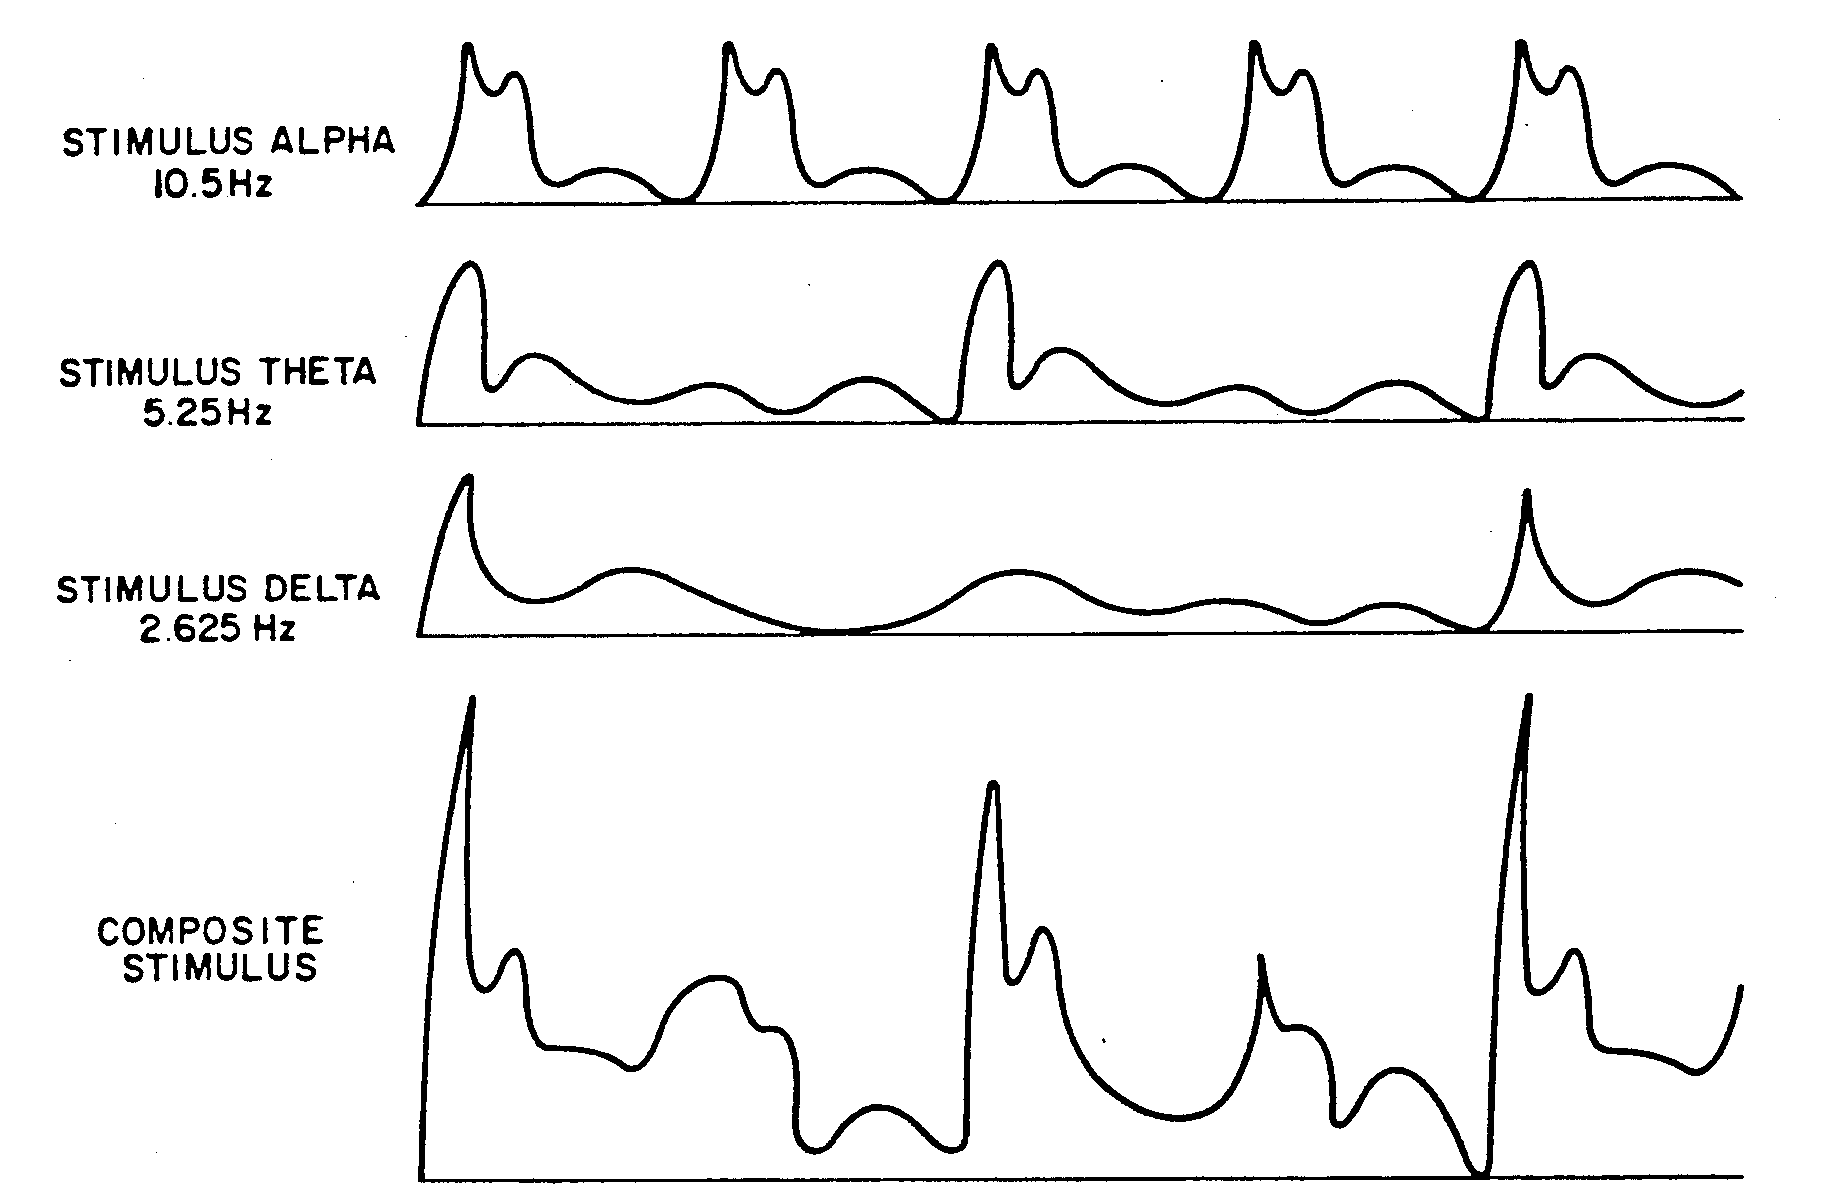
\includegraphics[width=350px]{BrainwaveComposition.png}
  \caption{A composition of alpha, theta and delta brainwaves. Credit: \cite{gall1992method}}
    \label{fig:brainwaveComposition}        
\end{figure}

\vspace{5mm}

Please note that almost always the EEG will display a composition of a set of types at any point in time. One example can be seen in the figure \ref{fig:brainwaveComposition}. Brain Computer Interfaces (BCIs) are a channel of communication between the electroencephalograph (EEG) and the computer.

